\subsection{Data transformations}\label{sec:transformaciones}

The analysis of ranges and normality shows that the quantitative variables
are markedly skewed and on heterogeneous scales, which, without prior
treatment, would distort the subsequent multivariate analysis. The
transformation decisions that produce the final dataset are documented
below.

The procedure covers all available quantitative variables; qualitative and
binary variables are excluded. \texttt{RAINF}, which measures precipitation
in mm/h, has a skewness of 144.85, far above the range of $-1.4$ to 13.3 of
the other variables. The cause is the disproportionate frequency of zeros,
since days without rain far outnumber days with rain: the variable is
classified as \textbf{zero-inflated} and requires a treatment different from
the rest. Instead, the binary variable \texttt{llovio} (it rained) is
derived, defined as

\begin{align}
     \texttt{llovio}=\begin{cases}
        0\;\texttt{RAINF} = 0\\
        1\;\texttt{RAINF} > 0
    \end{cases}
\end{align}

The criterion that determines whether a variable is transformed is

\begin{align}
    |\text{skewness}(x_i)|<0.5\,\forall\, x_i\in X\;\;i=1\,,2\,\dots,n
\end{align}

The Box-Cox transformation requires positive observations, so a prior shift
is applied to the variables that contain non-positive values:

\begin{align}
    \forall i\in X\;\forall j\in x_i\;x_{ij} \leq0 \implies x_i = x_i - \min{x} + 1
\end{align}

The skewness before and after the transformation is reported in
\cref{tab:sesgos-transformacion}.

\begin{table}[ht]
  \centering
  \caption{Skewness of each quantitative variable before and after the
    shifted Box-Cox transformation.}
  \label{tab:sesgos-transformacion}
  \begin{tabular}{lrr}
    \toprule
    Variable & Original skewness & Transformed skewness \\
    \midrule
    O3        & 1.28   & $-0.07$ \\
    CO        & 1.91   & 0.01 \\
    NO        & 6.87   & $-0.01$ \\
    NO2       & 1.91   & 0.02 \\
    NOX       & 4.49   & 0.00 \\
    SO2       & 13.31  & 0.00 \\
    PM10      & 3.66   & $-0.04$ \\
    PM2.5     & 5.70   & 0.09 \\
    TOUT      & $-0.43$ & $-0.06$ \\
    RH        & $-0.32$ & $-0.17$ \\
    SR        & 1.52   & 1.02 \\
    RAINF     & 144.85 & --\footnotemark \\
    PRS       & 0.09   & 0.00 \\
    WSR       & 6.89   & 0.10 \\
    viento\_u & $-1.42$ & 0.75 \\
    viento\_v & $-0.50$ & 0.62 \\
    O3\_8h    & 0.96   & 0.01 \\
    \bottomrule
  \end{tabular}
\end{table}
\footnotetext{\texttt{RAINF} was not transformed: being zero-inflated, its
skewness is not reduced by Box-Cox. It was replaced by the binary variable
\texttt{llovio}.}

Three variables do not meet the criterion after Box-Cox: \texttt{SR}, because
of the block of nighttime zeros (1.02), and the two wind components (0.75 and
0.62). They are kept because the daily aggregation of
\cref{sec:agregacion-diaria} summarizes them (cumulative radiation, vector
means), and on those summaries the same criterion is met, with re-estimated
parameters documented in \cref{tab:dic-diario-sesgo}.

After scaling ($z$-score), the densities of the variables are centered and
comparable with one another (\cref{fig:densidad-escaladas}).

\begin{figure}[ht]
  \centering
  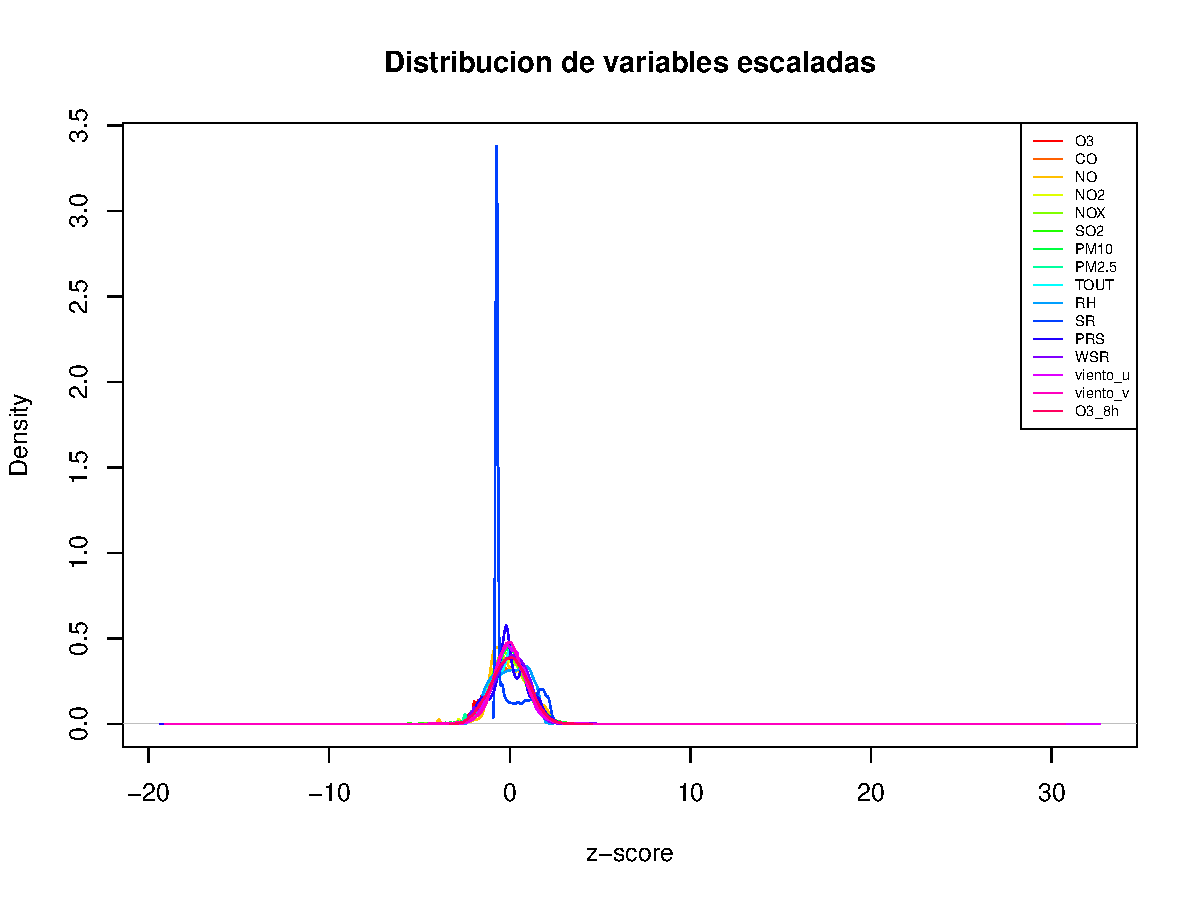
\includegraphics[width=\linewidth]{densidad_variables_escaladas.pdf}
  \caption{Distribution (density) of the quantitative variables after the
    Box-Cox transformation and scaling.}
  \label{fig:densidad-escaladas}
\end{figure}

The dictionary of the transformed dataset, with the full description of each
variable, its treatment and its skewness before and after, is given in
\cref{sec:diccionario-transformado}.
